\chapter{Silicon Photo-multipliers fundamentals}
\label{ch:background}
In this chapter, the fundamentals of silicon photo-multipliers will be reviewed. The material described is focused of the physics behind the SiPM starting from the PN junction to the Diodes and then the SiPM.

%
% Section: Basic principles
%
\section{PN junctions}
\label{sec:background:Basic principles:PN junctions}
A PN junction is formed by combining two semiconductor materials which have been doped differently. Doping involves introducing impurities (group III elements for positive doping and  group V for negative doping) into the crystal structure, creating free charge carriers. The P-type semiconductor contains positive charge carriers called holes. The other material, the N-type semiconductor, has an excess of negative charge carriers called electrons. 

When a P-doped crystal is joined with an N-doped crystal, a depletion region is created by the diffusion of the charge carriers. The holes from the P-type material and the electrons from the N-type material combine. As a consequence of this recombination, positive electric charge accumulates on the N-doped side, while negative electric charge accumulates on the P-doped side. This charge generates an electric field in the depletion region and therefore a voltage, referred to as built-in voltage. One can see In Fig. \ref{fig:PN junctions scheme} a scheme of a P and N type material and a PN junction. 
\begin{figure}[htbp]
 \centering
 \includegraphics[width=0.6\textwidth]{gfx/schemes/PN_junction.png}
 \caption{PN junction scheme, before joining the two materials (top) and after (bottom). }
\label{fig:PN junctions scheme}
\end{figure}


\section{Diode}
\label{sec:background:Basic principles:Diodes and photo-diodes}
A diode is an electronic component made of a PN junction. 
When an external voltage is applied, we referred to it as the bias voltage $V_{bias}$, the size of the depletion region can vary and so the diode current. The IV characteristic curve of a diode is shown in Fig. \ref{fig:chapter02:Diodes and photo-diodes: iv curve}. Depending on the direction of the bias voltage, one can see different behaviors, and define the different operation modes. 
\begin{figure}[htbp]
 \centering
\includegraphics[width=0.7\textwidth]{gfx/documentation/Diode_IV_curve.png}
 \caption{Diode IV characteristic curve \cite{DiodeCurve}.}
 \label{fig:chapter02:Diodes and photo-diodes: iv curve}
\end{figure}


\paragraph{Forward Bias mode.} Forward bias means that the voltage applied reduces the width of the depletion region. The cathode is connected to the P-type and the anode to the N-type of the junction. More electrons will recombine with the holes in the P doped region, and holes will recombine in the N-type resulting in a smaller depletion.

\paragraph{Reverse Bias mode.} When a diode is in Reverse Bias mode, the cathode is connected to the N side (anode to the P side). Holes are attracted to the negatively charged end of the generator and electrons to the positively charged end resulting in a larger depletion region. 

\paragraph{Breakdown.} 
The breakdown voltage $V_{bd}$ is the bias voltage value where any free charge carrier in the depletion region is sufficiently accelerated by the electric field so that it triggers an avalanche. A single electron-hole pair can create a self-sustaining electron-hole avalanche. The regime of operation beyond the breakdown voltage ($V_{bias} > V_{bd}$) is often called Geiger-Mode and we can define a quantity named overvoltage $\Delta V = V_{bias}-V_{bd}$ for this regime.


\subsection{Photodiode}
\label{ch:2:subsec:Photodiode}
The standard photodiode is a PN junction. When a photon enters the detection area (depletion region), it can interact by photo-electric effect and create an electron-hole pair. If the diode is not biased, this electron pair will generate a small tension and behaves like a solar cell. Photodiodes are employed to measure light sources big enough so that the current produced is measurable. They are not suited to detect single photons. 

\subsection{Avalanche photodiode}
\label{ch:2:subsec:Avalanche photodiode}
An \ac{APD} is reverse biased but the electric field's intensity is high enough so that the electron can gain enough speed to ionise other atoms in the crystal and triggering a chain reaction or avalanche. Due to their higher effective mass, the holes are not accelerated enough to create an electron-hole avalanche because APDs operate below breakdown voltage. 

\section{Single Photon Avalanche Diodes}
\label{sec:background:Basic principles:SPADs}
\ac{SPAD} or \ac{G-APD} is an Avalanche Photo-diode operating in Geiger-Mode, meaning that the bias voltage is above the breakdown voltage. This specificity allows this device to detect single photons, since one pair of electron-hole can trigger a self-sustaining avalanche and then generate an electric current intense enough to be measured. Due to the exponential growth of the current generated, if nothing is done the quench it, the diode can be damaged or even burned. The quenching resistor $R_Q$ is introduced to prevent the diode from burning. When the photo-current $I_{ph}$ increases, the voltage at the ends of the resistor $R_Q$ increases (because $V_{R_Q}= R_Q\cdot I_{ph}$). By the law of mesh $V_{bias} + V_{diode}+ V_{R_Q} = 0$, hence $V_{diode}$ decreases as $V_{R_Q}$ increases. The voltage $V_{diode}$ will drop below $V_{bd}$ and the avalanche created will not be self-sustaining. The avalanche is then quenched.

\begin{figure}[htbp]
 \centering
\includegraphics[width=0.7\textwidth]{gfx/documentation/switch_analogy.png}
 \caption{SPAD response as function of $V_{bias}$. 
 \cite{Onsemi2021IntroductionMultipliers}
 }
\label{fig:chapter02:Diodes and photo-diodes:switch}
\end{figure}
The working principle is shown in Fig. \ref{fig:chapter02:Diodes and photo-diodes:switch}. 
When a photon is detected, an avalanche is triggered and then quenched. During this time, the SPAD recharges, avalanches could still be triggered, but will be smaller until the SPAD recharges. This time is defined as the recovery time $\tau_{rec}$. We can define another time constant of the pulse shape $\tau_{long}$ that corresponds to the time it takes for the signal to go down to the baseline and it is equal to the recovery or recharging time $\tau_{rec}$. A SPAD can detect single photons, but it will not be able to distinguish between two or more photons that hit within the recharging time. Once the avalanche is triggered, a second photon hit will not result in an avalanche twice as big. Nevertheless, there is a way to detect multiple photons, by adding several SPADs in parallel and form a SiPM.  
\begin{figure}[htbp]
    \centering
    \includegraphics[width=0.48\textwidth]{gfx/documentation/spad_circuit.png}
    \caption{SPAD electronic circuit equivalent, with integrated quenching circuit. 
    \cite{Gundacker2020TheDetector}}
\end{figure}


\section{Silicon Photo-Multiplier}
\label{sec:background:SiPMs}
The SiPM is a solid-sate photodetector made of multiple SPADs connected in parallel. It can detect multiple photons at once if they hit different pixels. One can see the electronic circuit of an example of SPAD array composing a SiPM.
\begin{figure}[htbp]
    \centering
    \includegraphics[width=0.5\textwidth]{gfx/schemes/sipm.drawio.pdf}
    \caption{SiPM electronic circuit equivalent with the SPADs connected in parallel.}
    \label{fig:chapter02:Sipm:electronic scheme}
\end{figure}


\subsection{Pixel or Micro-Cell}
\label{subsec:Pixel or Micro-Cell}
\begin{wrapfigure}[12]{r}{0.4\textwidth}
    \centering
    \includegraphics[width=0.4\textwidth]{gfx/documentation/pixel_pic.png}
    \caption{Image of a pixel structure on a SiPM \cite{Onsemi2021IntroductionMultipliers}.}
    \label{fig:chapter02/sipm/pixel pic}
\end{wrapfigure}
In a SiPM, each SPAD is a pixel (or micro-cell). The structure of a pixel, including its active and inactive areas, is depicted in Fig. \ref{fig:chapter02/sipm/pixel pic} where the internal square is the active area. The borders contain the trenches, quenching resistors and referred to as the inactive area. When designing a SiPM, manufacturers can produce SiPMs with different number of pixels and pixel sizes. For a given detector size, these two parameters have advantages and drawbacks. 
Increasing the number of pixels while maintaining a constant detector size enhances the dynamic range. The dynamic range can be analogously understood as the resolution of the detector, a smaller dynamic range reduces the chances that two close photons hit two different pixels.
However, with smaller pixels, the two photons might hit separate pixels, enabling their individual counting.
There is a trade-off when increasing the number of pixels, as it also increases the inactive area. This inactive area consists of components such as quenching resistors, trenches, metal guards, etc. The ratio between the active area and the total area is defined as the \ac{FF}. The FF significantly influences the PDE, as explained below in \ref{subsection:PDE}.
Therefore, for a detector of the same size, increasing the number of pixels enhances the dynamic range but reduces the gain and PDE and vice versa.


\subsection{Gain}
\label{subsection:Gain}
The gain of a SiPM is defined as the amount of electron-hole pairs generated in an avalanche. It represents the avalanche size and is proportional to the active volume in the pixel.
The gain is computed as in Eq. \eqref{eq:gain theory} (where $C_d$ is the pixel capacitance): 
\begin{equation}
    G= \frac{C_d \cdot \Delta V}{e}
    \label{eq:gain theory}
\end{equation}


\subsection{Photo-detection efficiency }
\label{subsection:PDE}
PDE is a key characteristic of a SiPM and defines the probability that a photon is converted into signal. This quantity depends on several parameters, such as the wavelength of the detected photons $\lambda$ or the overvoltage $\Delta V$. The formula is usually of the form:
\begin{equation}
      PDE(\lambda, \Delta V)= \eta(\lambda)\cdot \varepsilon(\Delta V)\cdot FF  
    \label{eq:pde theory}
\end{equation}
where $\eta(\lambda)$ is the quantum efficiency of the cell, which is the probability that a photon generates an electron-hole pair.   $\varepsilon(\Delta V)$ is the avalanche triggering probability and $FF$ the Fill Factor. 
% Vbd, R_Q, Gain, PDE

\subsection{Dark count and correlated noise}
\label{subsec:Correlated noise}
The avalanche triggering is not necessarily from a photon, an electron-hole pair can be created by thermal excitation resulting in noise. 
\paragraph{Dark count} Dark Counts or Dark Current are the primary source of noise in the SiPM. Some free charge carriers can be generated in the depletion region due to thermal excitation. Since the SiPM operates above $V_{bd}$, any single charge carrier can generate an avalanche.The pulse amplitude a of dark count is $1$\ac{PE} since only one pixel is fired. 

\paragraph{Optical Direct Cross talk} During an  avalanche, the accelerated electrons can emit photons by Bremsstrahlung effect. Those photons can travel and hit other pixels close by and in turn generate another avalanche. Hence the total signal will be the combination of the primary avalanche and the secondary avalanche from the Bremsstrahlung photon. Due to the small spatial distance between the pixels, there is approximately no delay between the signal from the primary photon and from the cross-talk photon, resulting in a 2PE peak. This type of noise is called \ac{DiXT} and we can see an example In Fig. \ref{fig:chapter02:Sources of noise}. First order DiXT is $2$PE in amplitude because two pixels are fired. There exist higher order DiXT corresponding to the number of pixels in the neighborhood fired but these are less common. 

\paragraph{Optical Delayed Cross talk}
\ac{DeXT} occurs when a photon from an avalanche generates an electron-hole pair outside the depletion region. Usually they will recombine but there is a probability that they don't. In this case, the charge carriers may drift towards the depletion region within a significant time interval. Once in the depletion region, they can trigger an avalanche in the other pixel resulting in a signal corresponding to a single photon detection with a $1$PE amplitude. 
% band gaps traps definition 

\paragraph{External Cross talk} External Cross talk is when a photon from an avalanche in one pixel is reflected by an additional coating on the top of the SiPM. This reflected photon can hit other pixels and generate this noise. In Fig. \ref{fig:all different cross talks} the different cross talk mechanisms are shown. 

\begin{figure}[htbp]
    \centering
    \includegraphics[width=\textwidth]{gfx/schemes/external_xTs.png}
    \caption{The three cross talk mechanisms in a SiPM \cite{ClaudioPiemonte2013PerformanceApplication}.}
    \label{fig:all different cross talks}
\end{figure}

\paragraph{After pulse}
The silicon crystal in the depletion region can have defects in their structure causing a change in the bands structure with a creation of a new level. An additional level, called a trap, may be created below the conduction band and can receive charge carriers created during a avalanche. After some time, the trapped charge carrier could be released by different effects such as thermal excitation or tunneling. Since the trap is in the depletion region, the now free charge carrier will be accelerated and may trigger an avalanche. 
\begin{figure}[htbp]
    \centering
    \includegraphics[width=0.6\textwidth]{gfx/documentation/afterpulse_example.png}
    \caption{Example of different after pulse shape and the fit of their amplitude, allowing to find $\tau_{rec}$. 
    \cite{Girard2018CharacterisationDistributions}}
  \label{fig:chapter02:Sources of noise: after pulse signal ex}
\end{figure}
The avalanche intensity will depend on the release time of the charge carrier meaning that the after pulse \ac{AP} signal can have different amplitude varying from $0$ to $1$ \ac{PE}. One can measure the recovery time $\tau_{rec}$ as shown in Fig. \ref{fig:chapter02:Sources of noise: after pulse signal ex}

\begin{figure}[htbp]
    \centering
    \includegraphics[width=0.9\textwidth]{gfx/documentation/noise_shapes.png}
    \caption{Example of different kind of noises shapes, and identification. 
    \cite{Gundacker2020TheDetector}
    }
    \label{fig:chapter02:Sources of noise}
\end{figure}

\section{Characterised detectors}
\label{ch:background:SiPM:characterised detectors}
This work studies three different detectors from FBK and one from Hamamatsu. 
\\
All SiPM arrays are composed of $128$ channels of \SI{250.4}{\micro m} wide. More specifications about these detectors are shown in Table \ref{table:detector specs}. A high definition picture of a SiPM from FBK is shown in \ref{fig:SiPM FBK}.
\begin{figure}[htbp]
    \centering
    \rotatebox{-90}{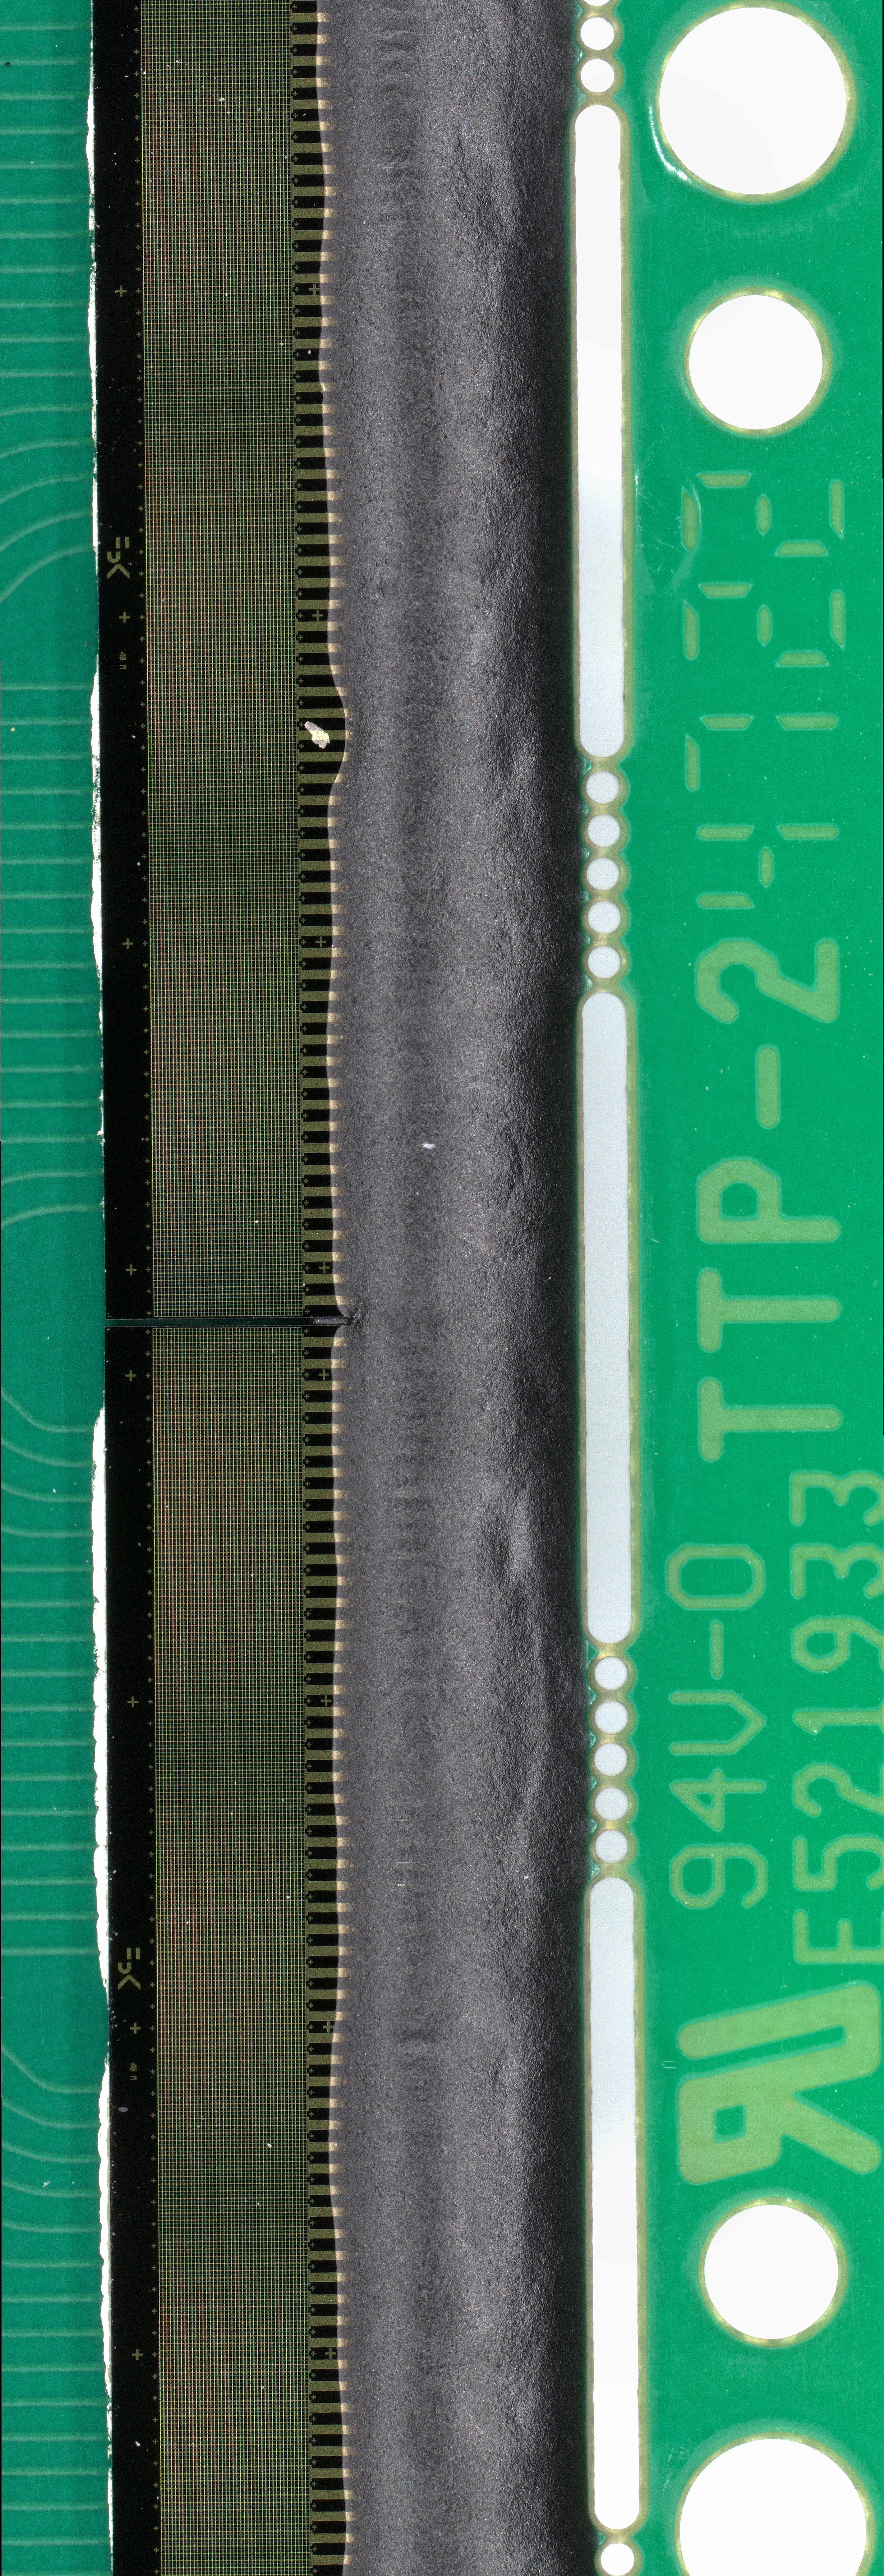
\includegraphics[width=0.35\textwidth]{gfx/pictures/SiPMarray.jpg}}
    \caption{128 channel SiPM array from FBK. Taken with a Keyance optical microscope, by G. Haefeli. }
    \label{fig:SiPM FBK}
\end{figure}
The Hamamatsu H2017, and the FBK \SI{31}{\micro m} \& \SI{42}{\micro m} have the same dimensions since they are designed to read out the light from the SciFi tracker. Another sample of the FBK \SI{31}{\micro m} is studied with an additional epoxy layer on the top of the sensitive area. 
\\
The characterised SiPMs from FBK are all from the same wafer, shown in Fig. \ref{fig:picture wafer} (a). In Fig. \ref{fig:picture wafer} (b), the SciFi A \& B correspond to the \SI{31}{\micro m} pixel size. The SciFi B is not analysed in this work. SciFi C is the SiPM with the largest pixel size of all three from FBK with \SI{42}{\micro m}. The \SI{16}{\micro m} (the one denoted \ac{ECAL} In Fig. \ref{fig:picture wafer} (b)) has a channel height bigger than the other ones because its use has a different purpose. In the ECAL, the fibre mats has a larger thickness, hence the choice of having SiPMs wider to collect all the photons. The Hamamatsu detector's breakdown voltage has a temperature dependency of \SI{54}{\milli \volt. \per \celsius}\cite{HamamatsuPhotonicsHowPhotonics} whereas the FBK have \SI{32}{\milli \volt. \per \celsius}.

\begin{table}[h]
\centering
\begin{tabular}{|l|l|l|l|l|l|}
\hline
\textbf{SiPM}               & \textbf{H2017} & \textbf{FBK \SI{16}{\micro m}} & \textbf{\begin{tabular}[c]{@{}l@{}}FBK \SI{31}{\micro m} \end{tabular}}  & \textbf{FBK \SI{42}{\micro m}} \\ \hline
\textbf{Pixel size [\SI{}{\micro m}]}         &    $57.5 \texttt{x}62.5$ &  $15.65$   &  $31.3$ &   $41.733$           \\ \hline
\textbf{$N_{pixel}$ (per channel)}        &  $104$   &    $3072$    &  $424$    &     $234$    \\ \hline
\textbf{Channel active height [\SI{}{\micro m}]}     & $1658.9$  &   $3004.8$  &  $1658.9$  & $1627.6$   \\ \hline
\end{tabular}
\caption{Specifications of the studied detectors.}
\label{table:detector specs}
\end{table}

\begin{figure}[htbp]
  \centering
  \begin{subfigure}[b]{0.48\linewidth}
    \centering
    \includegraphics[width=0.9\linewidth]{gfx/pictures/Wafer.png}      
    \caption{}
  \end{subfigure}
  \hfill
  \begin{subfigure}[b]{0.48\linewidth}
    \centering
    \hspace{0.5cm}
    \includegraphics[width=0.7\linewidth]{gfx/pictures/FBK_types_Wafer.png}
    \caption{}    
  \end{subfigure}
    \caption{Picture of the FBK wafer containing the 4 types of detectors (a) and zoomed in picture of the 4 detectors types (b).}
    \label{fig:picture wafer}
\end{figure}

\subsection{Hamamatsu and FBK technology}
\label{ch:background:SiPM:characterised detectors:FBKvsH}

\paragraph{FBK NUV-HD technology}
The FBK \ac{NUV-HD} technology has been designed to have a high dynamic range, low correlated noise and to be used in cryogenic applications. The pixel edges contains a trench between active areas (in grey Fig. \ref{fig:fbk tech scheme trench photo} (a)) of less than \SI{3}{\micro m}. They reduce the probability of cross talk while limiting the dead space. A micro graph of these deep trenches can be seen in Fig. \ref{fig:fbk tech scheme trench photo} (b). The integrated poly-silicon quenching resistor can been In Fig. \ref{fig:fbk tech scheme trench photo} (a). An annotated picture of the FBK pixel is shown in \ref{fig:fbk tech scheme trench photo} (c) where the metal guards are visible. 
\begin{figure}[htbp]
  \centering
  \begin{subfigure}[b]{0.48\linewidth}
    \includegraphics[width=1\linewidth]{gfx/schemes/FBK_technology_spad.png}
    \caption{}  
  \end{subfigure}
  \hfill
  \begin{subfigure}[b]{0.48\linewidth}          
    \includegraphics[width=1\linewidth]{gfx/pictures/FBK_trench.png}  
    \caption{}
  \end{subfigure}
  \hfill
  \begin{subfigure}[b]{1\linewidth}          
    \includegraphics[width=1\linewidth]{gfx/pictures/FBK_techpic.png} 
    \caption{}
  \end{subfigure}
    \caption{Scheme of FBK cell (a) and photograph of FBK deep trenches between pixels (b) and view from above (c). \cite{Paternoster2019SiliconPerspectives}}
    \label{fig:fbk tech scheme trench photo}
\end{figure}


\paragraph{Hamamatsu technology}
A picture of the H2017 pixels shows the structure of this detector (see Fig. \ref{fig:H2017 pixels picture guido}). As in the FBK, trenches between the pixels are visible. On the Hamamatsu the $R_Q$ is composed of a thin transparent film on the active surface where as the FBK $R_Q$ is made of poly silicon. More informations about this detector can be found in \cite{SurfaceArray}.
\begin{figure}[htbp]
    \centering
    \includegraphics[width=0.8\textwidth]{gfx/pictures/H2017 pixels.jpg}
    \caption{Picture of the H017 detector's pixels with a Keyance optical microscope taken by G. Haefeli. }
    \label{fig:H2017 pixels picture guido}
\end{figure}
%no trenches
%what's it specifity? 




